\documentclass{beamer}
\usetheme{ensam}
\usepackage{pgfplots}
\usepackage{subcaption}
\usepackage{acronym}
\usepackage{tikz}
\usetikzlibrary{calc}
\usepackage{amsmath}
\usepackage {algorithmic}
\usepackage{algorithm}
\usepackage{eqparbox}
\usepackage[pdf]{graphviz}
\usepackage[font=scriptsize]{caption}
\usetikzlibrary{bayesnet,positioning,calc}
\tikzstyle{obs} = [latent,fill=lightBlue]
\tikzstyle{default}=[draw=sexyRed,thick,rounded corners,text width=0.5in,font=\scriptsize,align=center]
\usepgfplotslibrary{colorbrewer}
\usetikzlibrary{decorations.pathmorphing}
\definecolor{ForestGreen}{RGB}{34,139,34}
\newcommand{\comment}[1]{\textcolor{ForestGreen}{#1}}
%algorithmic comment
\renewcommand\algorithmiccomment[1]{%
  \hfill\comment{\#\scriptsize\eqparbox{COMMENT}{#1}}%
}
\renewcommand{\algorithmicrequire}{\textbf{Input:}}
\renewcommand{\algorithmicensure}{\textbf{Output:}}
\title{Stratégie d'exploration non informée}
\author{\underline{A.Belcaid}}
\institute{\small ENSA-Fès} 

%tikz bayesian theme
\usetikzlibrary{bayesnet,positioning,calc}
\tikzstyle{obs} = [latent,fill=lightBlue]
\tikzstyle{default}=[draw=sexyRed,thick,rounded corners,text width=0.5in,font=\scriptsize,align=center]
\DeclareMathOperator{\argmin}{argmin}

\pgfplotsset{every tick label/.append style={font=\tiny}}



%acronyms
% add bibliography
\usepackage[style=authoryear]{biblatex}
\renewcommand*{\nameyeardelim}{\addcomma\addspace}

\begin{document}
\maketitle

\begin{frame}
\begin{columns}
  \begin{column}{0.6\textwidth}
    {
      \begin{enumerate}
        \item Agent de résolution de problèmes.\\[0.5cm]
        \item Recherche des solutions\\[0.5cm]
        \item Exploration non informée
          \begin{itemize}
            \small
            \item Recherche en profondeur (DFS)\\[0.2cm]
            \item Recherche en largueur  (BFS)\\[0.2cm]
             \item Recherche uniforme en coût (UCS).
          \end{itemize}
      \end{enumerate} 
    
    }
  \end{column}
  \begin{column}{0.4\textwidth}
  \centering
  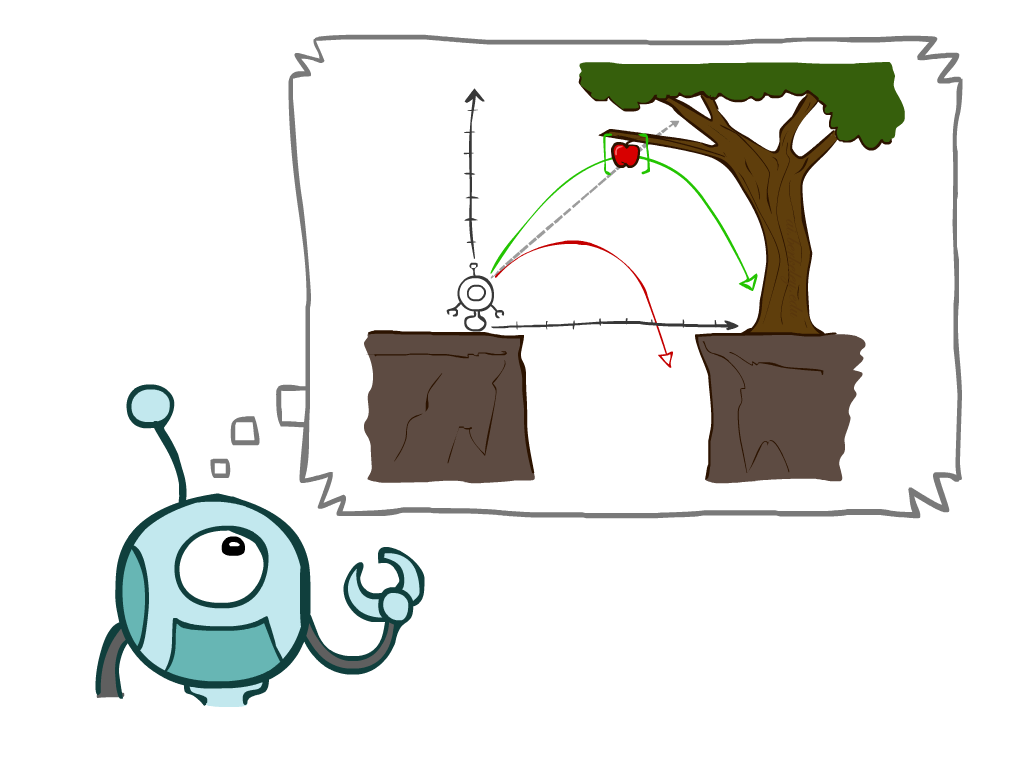
\includegraphics[width=5cm,height=5cm]{./images/agent_contents.png}
  \end{column}
\end{columns}
\end{frame}



%%%%%%%%%%%%%%%%%%%%%%%%%%%%%%%%%%%%%%
%  Agents et résolution de problèms  %
%%%%%%%%%%%%%%%%%%%%%%%%%%%%%%%%%%%%%%
\section{Agents de résolution de problèmes}%
\label{sec:agents_de_resolution_de_problemes}

\begin{frame}[t]{Agents réflexes}
  
  \begin{columns}
    \begin{column}{0.5\textwidth}
      
      \alert{\textbf{Agents réflexes}}:
    
      \begin{itemize}
        \scriptsize
      \item<2-> Choix d'action sur l'état actuel des perceptions avec une
        mémorisation.\\[1cm]
      \item<3->  L'environnement est soit stocké \textbf{entièrement} en
        mémoire, soit connait l'état actuel.\\[1cm]

      \item<4-> Ne considèrent pas les \alert{\textbf{conséquences}} de leurs actions.
      \end{itemize}
    \end{column}
    \begin{column}{0.5\textwidth}
      \only<1->{
        \centering
  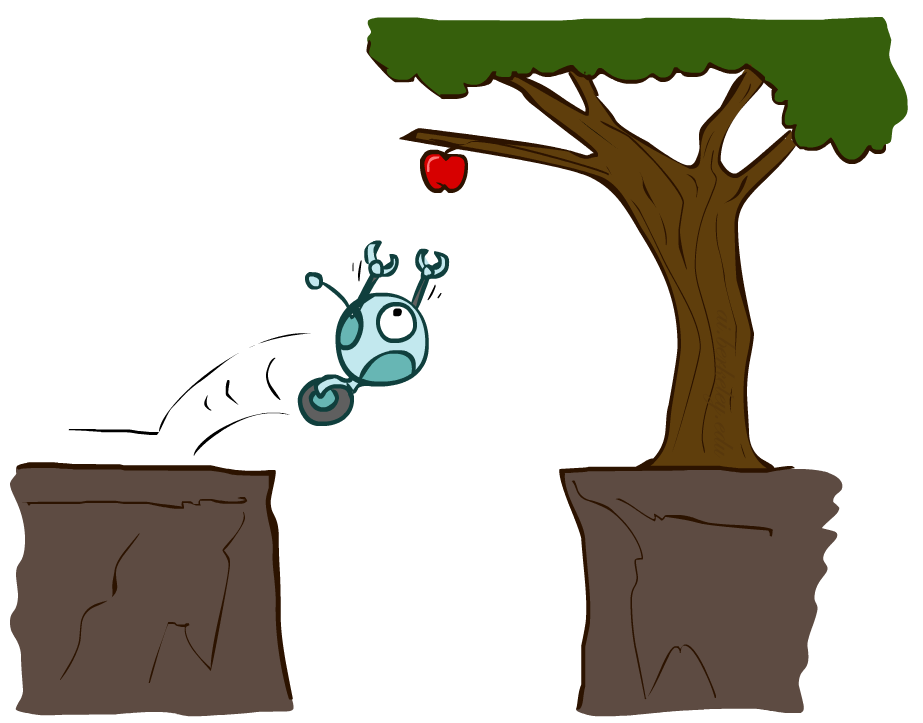
\includegraphics[width=5cm,height=5cm]{./images/reflex_agent_01.png}
      }
    \end{column}
  \end{columns}

  \vspace*{1cm}

  \only<5>
{
  \begin{block}{}
   \large \centering
   Est ce que les agents réflexes peuvent être \textbf{rationnels}?
  \end{block}
}
\end{frame}

%%%%%%%%%%%%%%%%%%%%%%%%%%%%
%  Agent de planification  %
%%%%%%%%%%%%%%%%%%%%%%%%%%%%

\begin{frame}[t]{Agents de planification}
  
  \begin{columns}
    \begin{column}{0.5\textwidth}
      
      \alert{\textbf{Agents de planification}}:
    
      \begin{itemize}
        \scriptsize
      \item<2-> Choix d'action selon une \alert{séquence} d'actions qui
        permettent d'attendre un \textbf{objectif}. \\[1cm]
      \item<3->  Utilisent une représentation \textbf{atomique} de
        l'environnement (connaissent l'état après le choix d'une action).\\[1cm]

      \item<4-> Doivent formuler un \alert{\textbf{objectif}} à
        atteindre.\\[1cm]
      \item<5-> Considèrent l'environnement  dans l'état actuel et
        \alert{future}.
      \end{itemize}
    \end{column}
    \begin{column}{0.5\textwidth}
      \only<1->{
        \centering
  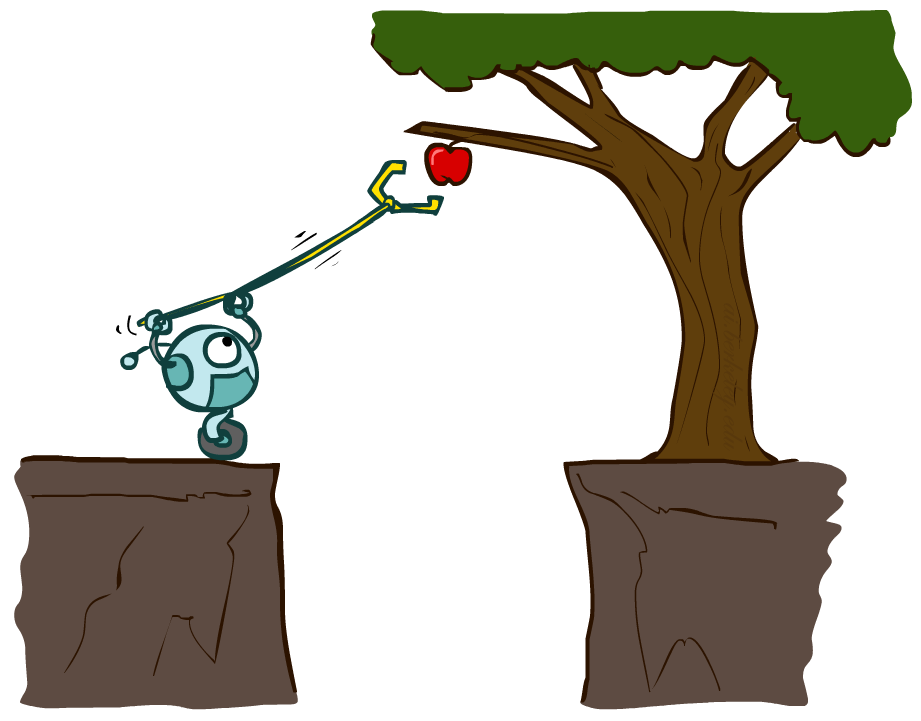
\includegraphics[width=5cm,height=5cm]{./images/planning_agent_01.png}
      }
    \end{column}
  \end{columns}
  \vspace*{1cm}
\end{frame}

\begin{frame}[t]{Quiz 1}
  Dans chacune des descriptions suivantes des \textbf{agents}, sélectionner leur
  \textbf{\alert{type}}:
  \begin{block}{Partie 1}
    \scriptsize
    Un agent Pacman qui est programmé à se déplacer toujours vers la
    \textbf{pellule} la plus proche.
    \begin{itemize}
      \tiny
      \item[$\square$] Agent réflexe
      \item[$\square$] Agent de planification 
    \end{itemize}
  \end{block}
  \pause

  \begin{block}{Partie 2}
    \scriptsize
    Un agent Pacman qui est programmé à se déplacer toujours vers la
    \textbf{pellule} la plus proche sauf s'il y as \textbf{fantôme} qui est à
    trois pas.
    \begin{itemize}
      \tiny
      \item[$\square$] Agent réflexe
      \item[$\square$] Agent de planification 
    \end{itemize}
  \end{block}
  \pause
  \begin{block}{Partie 3}
    \scriptsize
    Un système de navigation qui considèrent toutes les voix vers une
    \textbf{destination}. Puis il choisit la plus courte. 
    \begin{itemize}
      \tiny
      \item[$\square$] Agent réflexe
      \item[$\square$] Agent de planification 
    \end{itemize}
  \end{block}
\end{frame}
%%%%%%%%%%%%%%%%%%%%%
%  Search problems  %
%%%%%%%%%%%%%%%%%%%%%
\section{Recherche des solutions}%
\label{sec:recherche_des_solutions}

\begin{frame}[t]{Problème d'exploration}
  
\centering
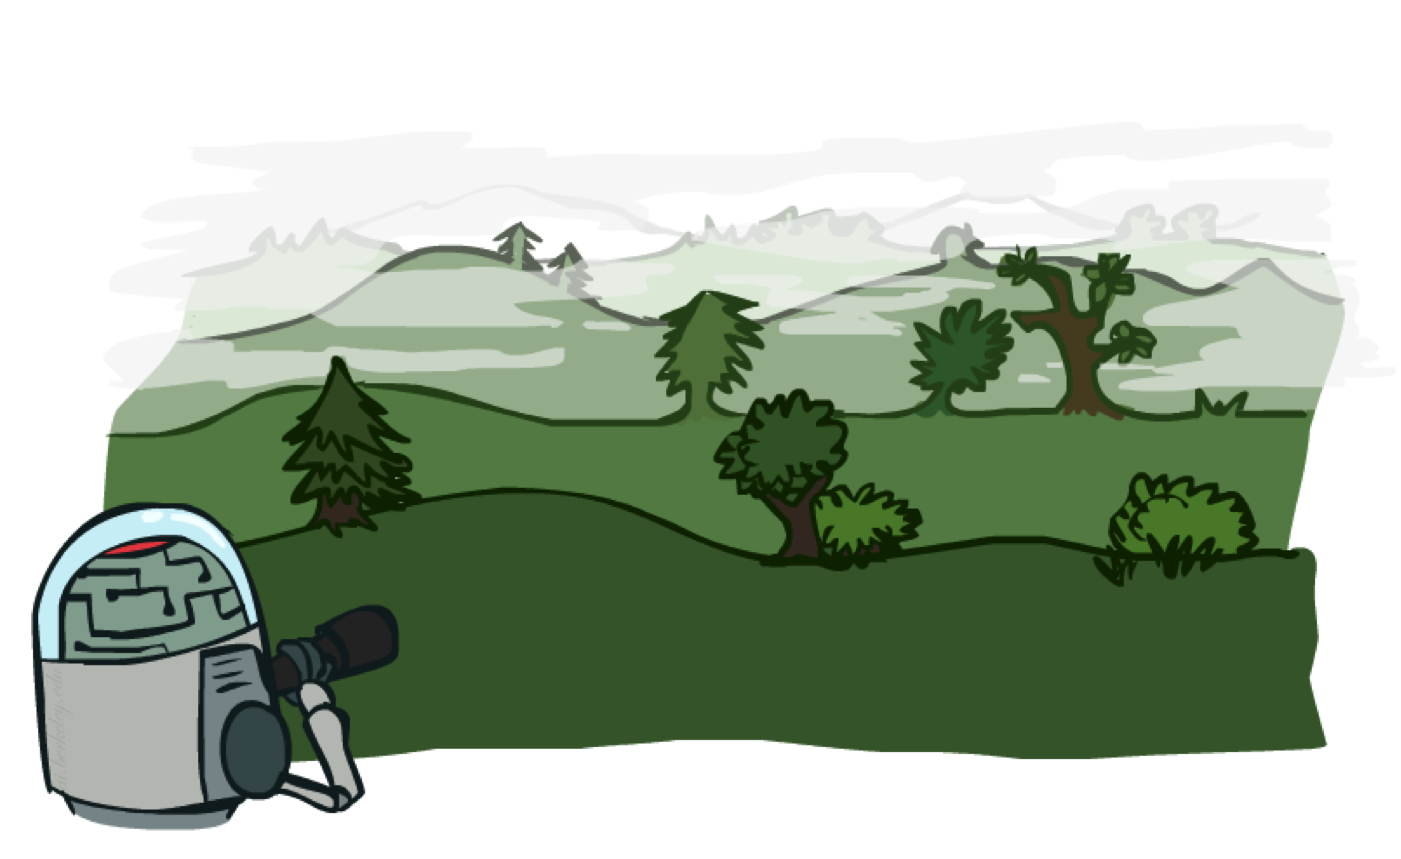
\includegraphics[width=0.8\textwidth,
height=0.8\textheight]{./images/search_logo.png}
\end{frame}


\begin{frame}[t]{Problème d'exploration}
  
\small
\centering
Un \textbf{\alert{Problème d'exploration}} consiste de:
\begin{itemize}
\item \textbf{Un espace des états} : \begin{tikzpicture}[scale=0.8]
      \node (s1){
\includegraphics[width=0.9cm,height=0.9cm]{./images/state_01.png}};
      \node[left of=s1](s2){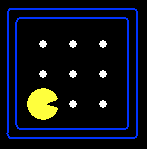
\includegraphics[width=0.9cm,height=0.9cm]{./images/state_02.png}};
      \node[left of=s2](s3){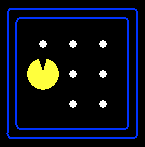
\includegraphics[width=0.9cm,height=0.9cm]{./images/state_03.png}};
      \node[left of=s3](s4){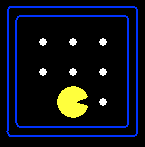
\includegraphics[width=0.9cm,height=0.9cm]{./images/state_04.png}};
      \node[left of=s4](s5){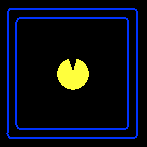
\includegraphics[width=0.9cm,height=0.9cm]{./images/state_05.png}};
      \node[left of=s5](s6){
\includegraphics[width=0.9cm,height=0.9cm]{./images/state_06.png}};
      \node[left of=s6](s7){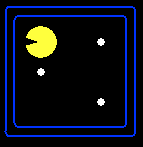
\includegraphics[width=0.9cm,height=0.9cm]{./images/state_07.png}};
    \end{tikzpicture}
  \pause
\item Fonction de \textbf{\alert{Succession}} (\emph{Action, Coût}):

  \pause
  \begin{tikzpicture}[yscale=0.7]
  \node at (0,0) (s1){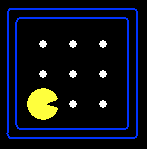
\includegraphics[width=0.9cm,height=0.9cm]{./images/state_02.png}};
\pause
\node at (4,1)(s2){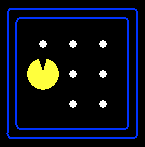
\includegraphics[width=0.9cm,height=0.9cm]{./images/state_03.png}};
\node at (4,-1)(s3){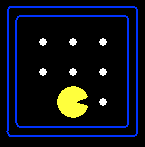
\includegraphics[width=0.9cm,height=0.9cm]{./images/state_04.png}};
\path[->,draw](s1)--node[above]{\scriptsize N, 1.0}(s2);
\path[->,draw,label=](s1)--node[below]{\scriptsize S, 1.0}(s3);

\end{tikzpicture}
\pause
\item Un état de \textbf{Départ}  et  un \textbf{\alert{Objectif}}.
\end{itemize}
\pause
Une \textbf{Solution} est un séquence d'action ( \textbf{\alert{Plan}}) pour
attendre l'objectif depuis l'état initial. 
\end{frame}


\begin{frame}[t]{Complexité du modèle}
  
  \centering
  Un problème d'exploration doit considérer un \textbf{\alert{Modèle}}:
  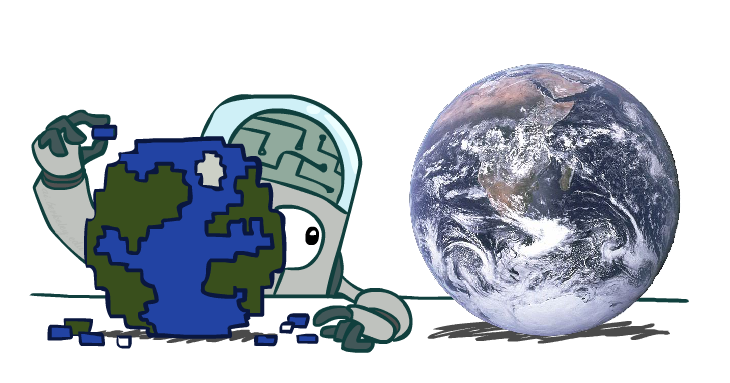
\includegraphics[width=9cm,height=0.6\textheight]{./images/exploration_model.png}
\end{frame}


\begin{frame}[t]{exemple: Recherche de chemins}
 \begin{columns}
   \begin{column}{0.7\textwidth}
    \centering 
    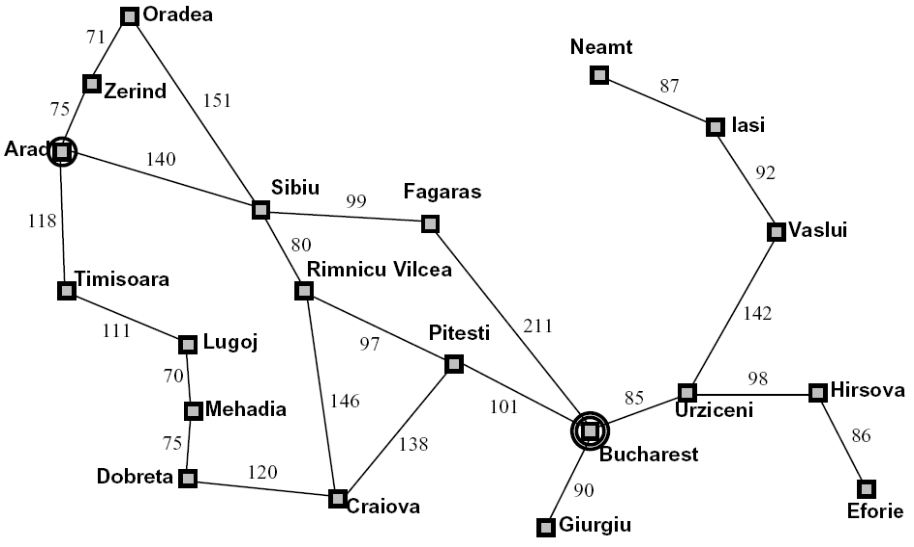
\includegraphics[width=0.8\textwidth,height=0.7\textheight]{./images/worlmap_model.png}
   \end{column}
   \begin{column}{0.3\textwidth}
     \begin{itemize}
       \scriptsize
     \item<1-> \textbf{Espace d'états}
         \begin{itemize}
           \item<2-> \alert{Villes}
         \end{itemize}
       \item<3-> \textbf{Fonction succession} :
         \begin{itemize}
           \tiny
           \item<4-> \alert{Chemin sortant d'une ville, coût est la distance}
         \end{itemize}
       \item<5-> \textbf{Etat de départ et Objectif}:
          \begin{itemize}
            \scriptsize
            \item<6-> \alert{Argad, Bucharest}
          \end{itemize}
        \item<6-> \textbf{Solution ?} 
          \begin{itemize}
            \scriptsize
            \item<7-> \alert{Chemin}
          \end{itemize}
     \end{itemize}
   \end{column}
 \end{columns} 
\end{frame}

\begin{frame}[t]{Espace d'état}
  
  \begin{block}{}
    \scriptsize
    l'\alert{espace des états} doit inclure \textbf{tous}  les détails de
    l'environnement.
    \centering
  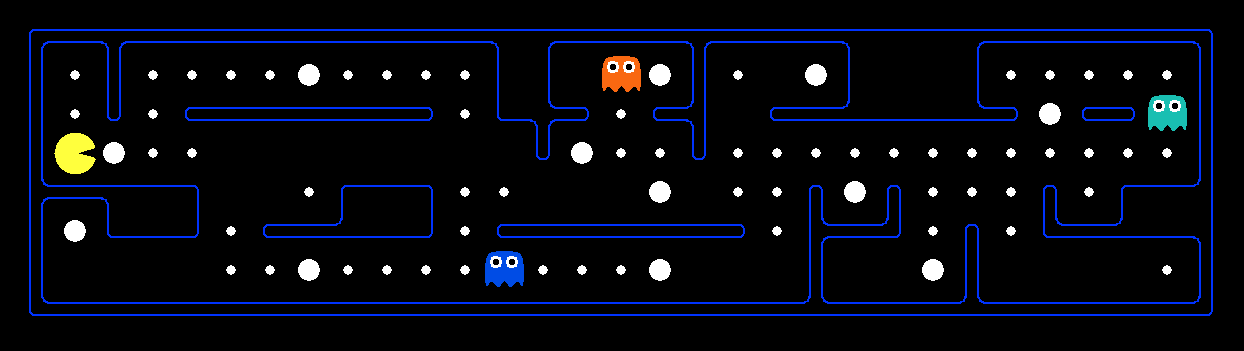
\includegraphics[width=5cm,height=2cm]{./images/world_state_contents.png}
  \end{block}
  \pause
  \begin{block}{}
    \centering
    \scriptsize
    Un \alert{état d'exploration} garde seulement les détails pour la
    planification (\emph{abstraction}) 
    \pause
    \begin{columns}
      \begin{column}{0.5\textwidth}
        \begin{itemize}
          \item Problem: chemin
            \begin{itemize}
              \footnotesize
            \item États:  positions $(x,y)$.
            \item Actions: NSEW
            \item Succession : nouvelle position
            \item Objectif: $(x,y)=\text{END}$
            \end{itemize}
        \end{itemize} 
      \end{column}
      \pause
      \begin{column}{0.5\textwidth}
        \begin{itemize}
          \item Problem: Manger tous les points.
            \begin{itemize}
              \tiny
            \item États:  positions $\{(x,y),\text{booléens des points}\}$.
            \item Actions: NSEW
            \item Succession : nouvelle position, mettre à jour les booléens
            \item Objectif: tous les booléens = Faux
            \end{itemize}
        \end{itemize} 
      \end{column}
    \end{columns}
  \end{block}
\end{frame}

\begin{frame}[t]{Cardinal de l'espace d'états}
  
  \begin{columns}
    \begin{column}{0.4\textwidth}
\centering      
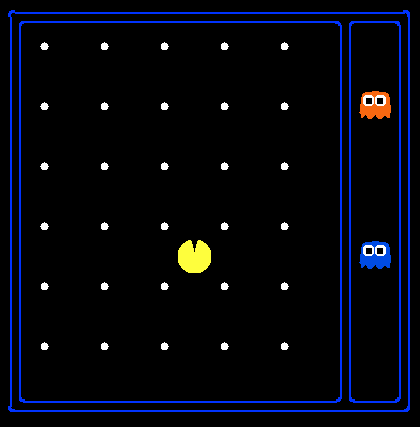
\includegraphics[width=4.5cm,height=4.5cm]{./images/state_space_count.png}
    \end{column}
    \begin{column}{0.6\textwidth}
      \begin{itemize}
        \scriptsize
        \item Espace d'état:
          \begin{itemize}
            \item Positions de l'agent: $\mathbf{120}$
            \item Position des points : $\mathbf{30}$
            \item Position des fantômes $\mathbf{12}$
            \item Action de l'agent : \textbf{NSEW} 
          \end{itemize}
        \item Cardinal espace d'état
          \pause
          \alert{
          \begin{equation*}
            120*2^{30}*12^2*4  
       \end{equation*}}
       \pause
     \item Cardinal (Chemin): 
       \begin{equation*}
         120
       \end{equation*}
       \pause
     \item Cardinal (Prendre tous les points)
       \begin{equation*}
         120*2^{30 }
       \end{equation*}
      \end{itemize}      
    \end{column}
  \end{columns}
\end{frame}


\begin{frame}[t]{Quiz 02 }
 \centering 
 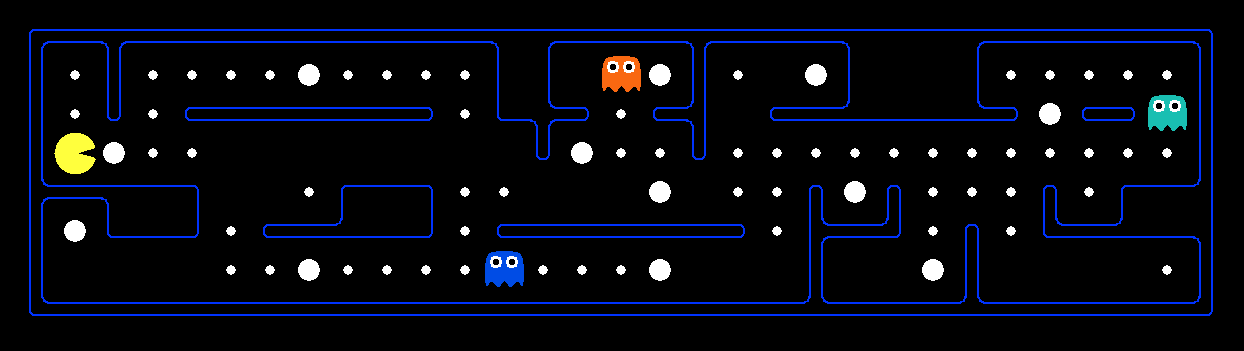
\includegraphics[width=0.9\textwidth, height=4cm]{./images/quiz_pacman_01.png}
 \begin{itemize}
   \item Le problème est de prendre tous les points, en gardant les fantômes en
     peur constante.
   \item Quelle sont les \alert{\textbf{informations}} à inclure dans votre
     espace d'exploration?
 \end{itemize}

 \pause
 \begin{columns}
   \begin{column}{0.5\textwidth}
     \begin{itemize}
       \scriptsize
       \item  Position Agent.
       \item Booléens des points
     \end{itemize}
   \end{column}
   \begin{column}{0.5\textwidth}
     \begin{itemize}
       \scriptsize
       \item Booléen des pullules de puissance.
         \item Temps restant de la cellule de puissance
     \end{itemize} 
   \end{column}
 \end{columns}
\end{frame}
%%%%%%%%%%%%%%%%%%%%%%%%%%%%%%
%  Exploration non informée  %
%%%%%%%%%%%%%%%%%%%%%%%%%%%%%%
\section{Exploration non informée}%
\label{sec:exploration_non_informee}
\begin{frame}[t]{Graphe d'espace d'états}
 \centering 
 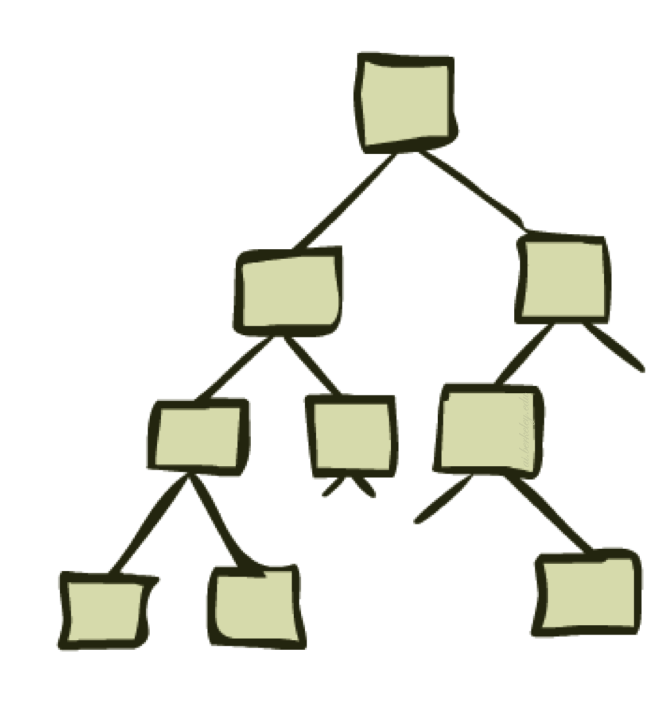
\includegraphics[width=0.7\textwidth,
 height=0.5\textheight]{./images/state_graph.png}
\end{frame}


\begin{frame}[t]{Graphe d'espace d'états}
  
  \begin{columns}
    \begin{column}{0.4\textwidth}
      \begin{itemize}
        \small
      \item<2-> \structure{\textbf{ Représentation
        mathématique}} 
        \begin{itemize}
          \scriptsize
        \item<3-> Les \alert{nœuds} sont des \textbf{abstractions} des
          configurations possible.
        \item<4-> Les \alert{arrêtes} sont des \textbf{successions}
          selon une \textbf{action} 
        \item<5-> Le nœud \alert{objectif} est un ensemble des nœuds
          du graphe.
        \end{itemize}
      \item<6-> Chaque configuration est \textbf{\alert{unique}}. 
      \item<7-> On peut \alert{rarement} construire un tel graphe. Mais il
        reste utile.
      \end{itemize}
    \end{column}
    \begin{column}{0.6\textwidth}
      \only<1-7>{
        \centering
 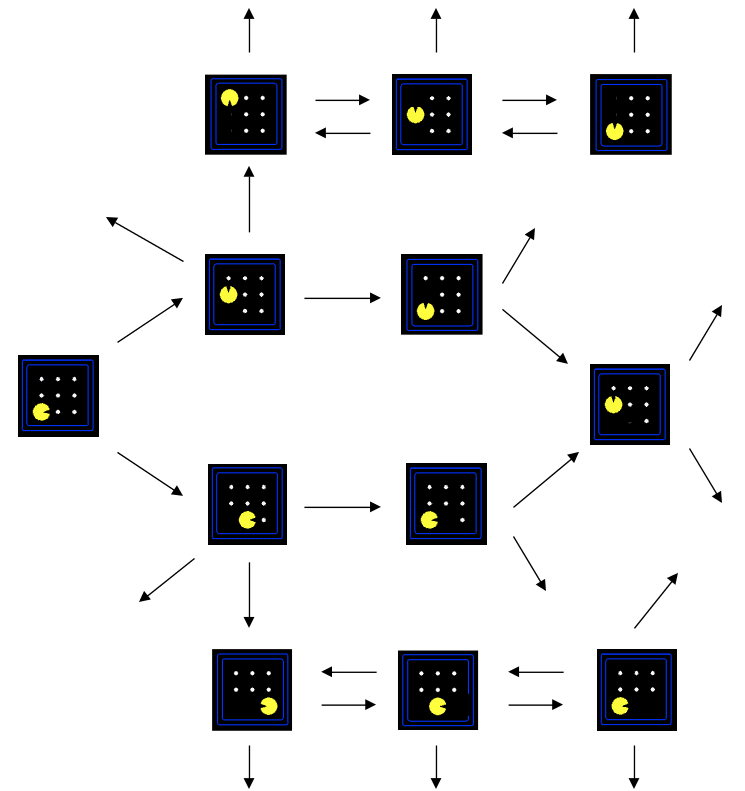
\includegraphics[width=0.7\textwidth,
 height=0.5\textheight]{./images/pacman_game_graph.png}
      } 
      \only<8>{
        \centering
 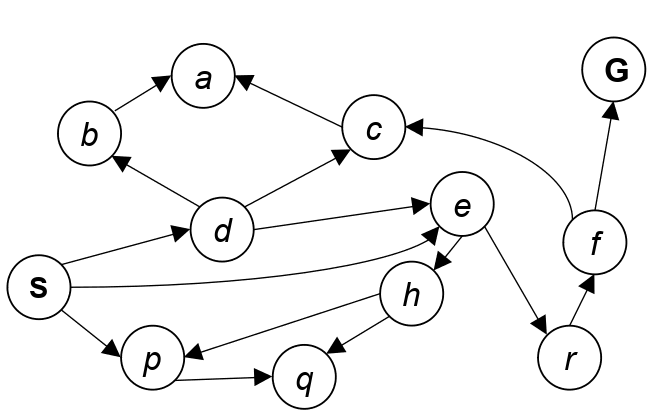
\includegraphics[width=1\textwidth,
 height=0.8\textheight]{./images/tiny_graphe.png}
      } 
    \end{column}
  \end{columns}
\end{frame}

\begin{frame}[t]{Arbre de recherche}
\begin{figure}[htpb]
\begin{center}
  \begin{tikzpicture}[xscale=1]
  \node (s) at (0,0) {
    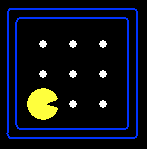
\includegraphics[width=0.6cm,height=0.6cm]{./images/state_02.png}
  }; 
  \node (s2) at (-2,-2) {
    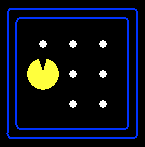
\includegraphics[width=0.6cm,height=0.6cm]{./images/state_03.png}
  }; 
  \node (s3) at (2,-2) {
    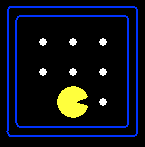
\includegraphics[width=0.6cm,height=0.6cm]{./images/state_04.png}
  }; 
\path[draw,->] (s1)--node[label=left :{N, 1} ]{} (s2);
\path[draw,->] (s1)--node[label=right :{E, 1} ]{} (s3);
\end{tikzpicture}
\end{center}
\end{figure}

\begin{block}{Arbre d'exploration}
  \begin{itemize}
    \footnotesize
  \item<2-> Liste des configurations possible suite à une \alert{action}.
  \item<3-> La \alert{\textbf{racine}} est l'état initial. 
  \item<4-> Les \alert{\textbf{fils}} sont les \textbf{successions}.
\item <5-> \alert{ \textbf{Noeuds}} sont des configurations avec un
  \textbf{plan}.(i.e meme configuration dans différents noeuds).  
\item<6-> \textbf{\alert{Pour la majorité des problèmes, impossible de
    construire toute
l'arbre}}.
  \end{itemize} 
\end{block}
\end{frame}




\begin{frame}[t]{Representation graph Vs Arbre}
 \begin{columns}
   \begin{column}{0.5\textwidth}
    \centering 
    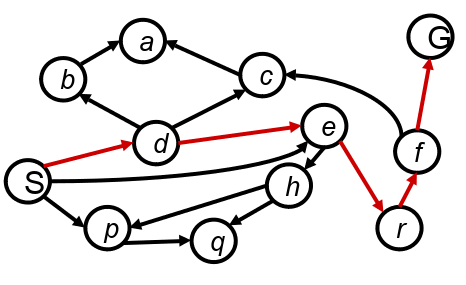
\includegraphics[width=5cm,height=5cm]{./images/graph_path_solution.png}
   \end{column}
   \begin{column}{0.5\textwidth}
     \centering
     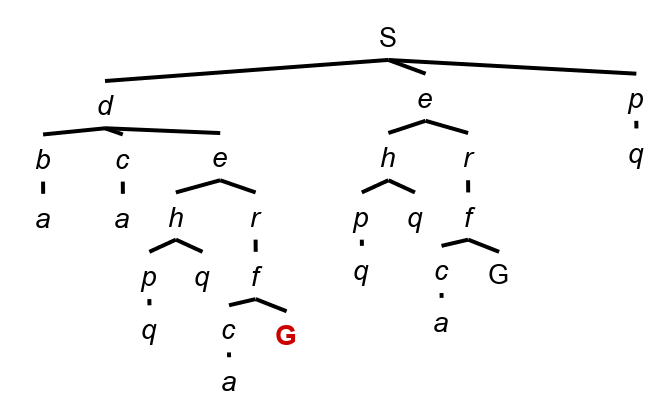
\includegraphics[width=5cm,height=5cm]{./images/tree_path_solution.png}
   \end{column}
 \end{columns} 
\pause
\begin{itemize}
  \small
\item Chaque noeud dans \textbf{l'arbre} est un chemin \alert{complet} au node initial.
\item L'arbre est construit \textbf{progressivement} par demande. 
\end{itemize}
\end{frame}

\begin{frame}[t]{Quiz 3}
 \begin{columns}
   \begin{column}{0.5\textwidth}
     \centering
      On considère le graphe d'états:\\
     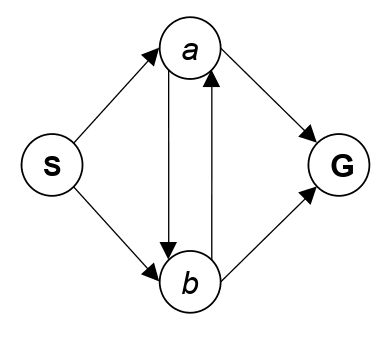
\includegraphics[width=5cm,height=5cm]{./images/four_state_graph.png}
   \end{column}
   \begin{column}{0.5\textwidth}
     Quelle est la \textbf{profondeur} de l'arbre d'exploration?\\[1cm]
\centering
\only<2->{\alert{ \Huge $\infty$ }}
     
   \end{column}
 \end{columns} 
\end{frame}

\begin{frame}[t]{Exemple Arbre d'exploration}
 \centering
 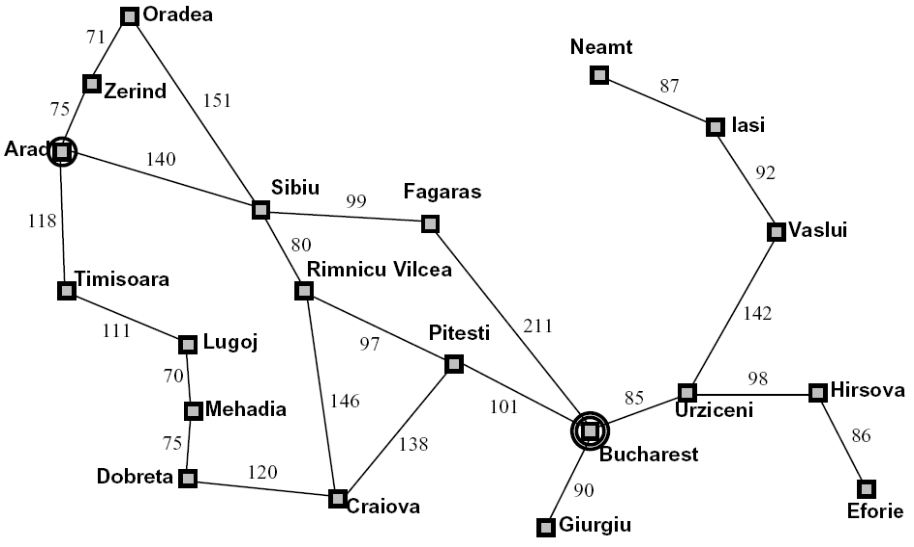
\includegraphics[width=10cm,height=8cm]{./images/worlmap_model.png}
\end{frame}


\begin{frame}[t]{Arbre d'exploration}
 \centering
 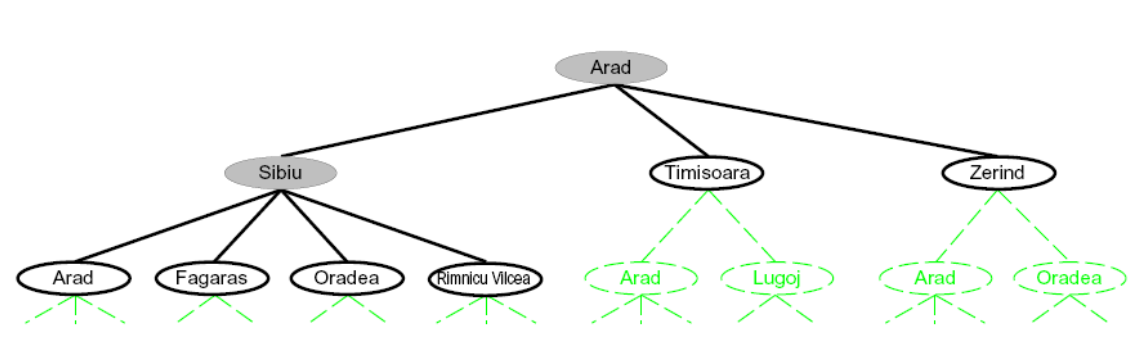
\includegraphics[width=10cm,height=4cm]{./images/world_map_first_tree.png}

\pause

\begin{block}{Exploration}
  \begin{itemize}
    \scriptsize
  \item Explorer des plans \emph{potentiels} (noeuds dans l'arbre).
  \item Maintenir une \textbf{\alert{frontière}} des plans partiels qui doivent
    être \textbf{considérés}.
  \item Explorer le \textbf{minimum} de neouds possibles.
  \end{itemize}

\end{block}
\end{frame}

\begin{frame}[fragile]{Algorithme général d'exploration d'arbres}
  \begin{algorithm}[H]
    \begin{algorithmic}
      \scriptsize
      \STATE \alert{Function}
        (\textbf{EXPLORER-ARBRE})(\emph{problème, stratégie})
     \STATE initaliser la frontière avec l'état initial. 
      \LOOP 
      \IF {frontière vide}  \RETURN\alert{échec}\COMMENT{Aucun noeud à explorer} \ENDIF
      \STATE \textbf{\structure{Choisir}} une feuille de la frontière selon
      \emph{statégie}
      \IF{feuille contient Objectif} \RETURN \alert{Succès}\COMMENT{Solution
      trouvée}.\ENDIF
      \STATE \alert{Développer} le noeud en ajoutant ces \alert{fils} à la
      frontière
      \ENDLOOP
    \STATE EndProcedure
  \end{algorithmic}
   \caption{Description informelle des algorithmes d'exploration en arbre} 
 \end{algorithm} 

 \begin{block}{Importants messages}
   \begin{itemize}
     \scriptsize
     \item Frontière
     \item Développement
     \item Stratégie d'exploration.
   \end{itemize}
 \end{block}
\end{frame}


\begin{frame}[t]{Exploration détaillée}
 \centering 
 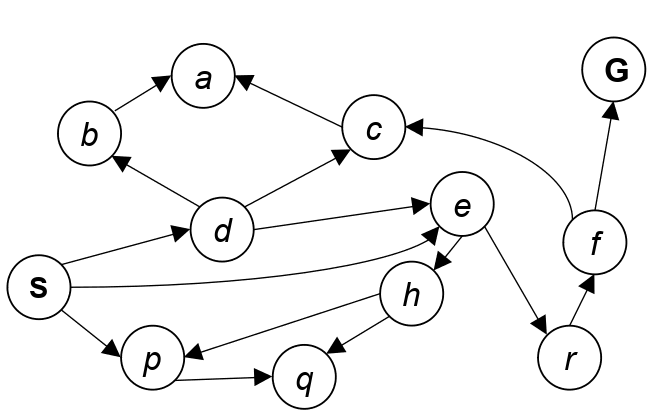
\includegraphics[width=6cm,height=5cm]{./images/tiny_graphe.png}
\end{frame}
%%%%%%%%%%%%%%%%%%%%%%%%%%%%%
%  Recherche en profondeur  %
%%%%%%%%%%%%%%%%%%%%%%%%%%%%%
\subsection{Recherche en profondeur (DPS)}%
\label{sub:recherche_en_profondeur_dps_}
\begin{frame}[t]{Depth First Search (Recherche en profondeur)}
 
  \centering
  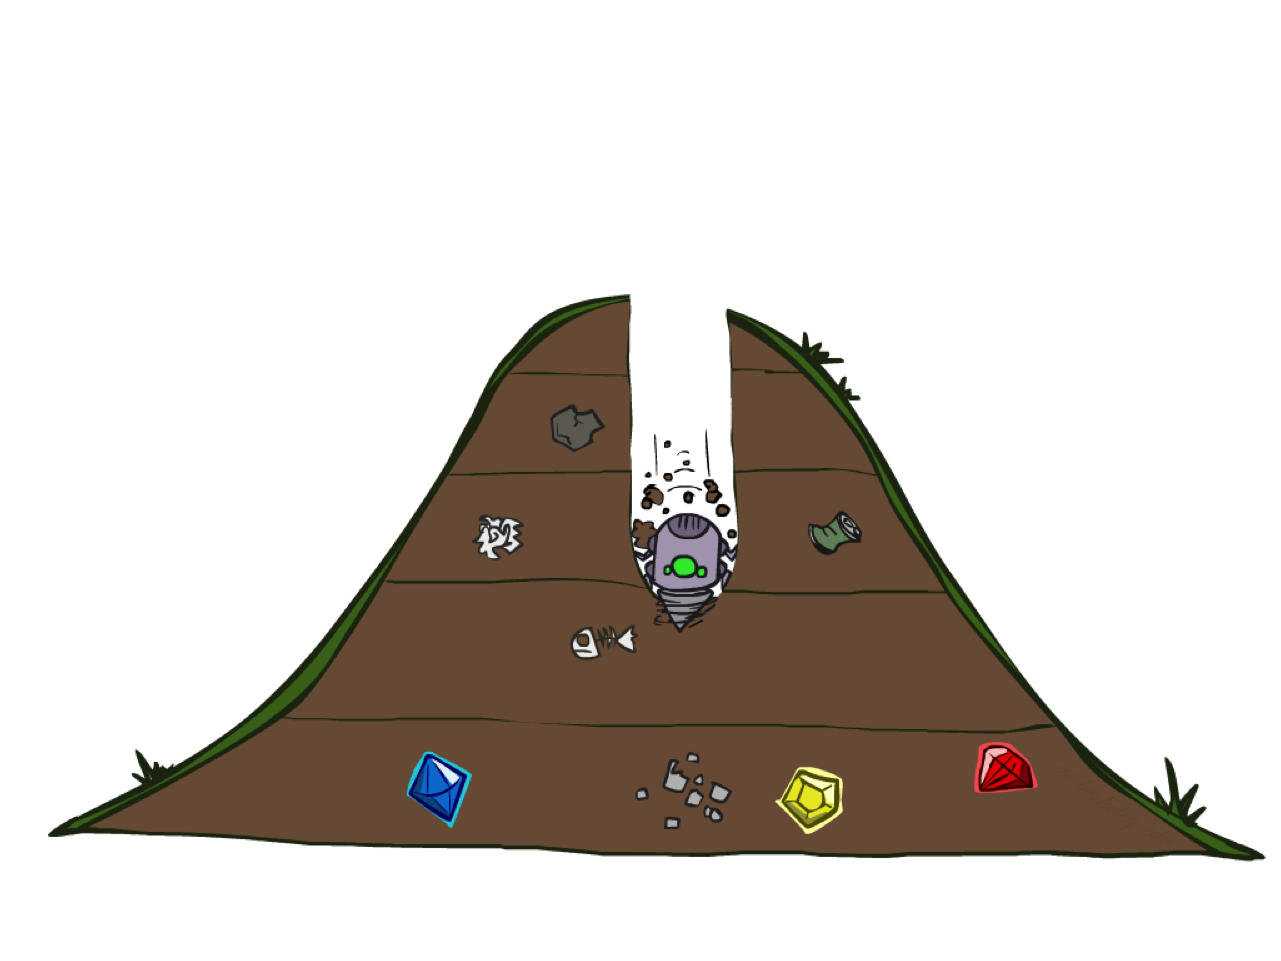
\includegraphics[width=8cm,height=6cm]{./images/depth_first_search.png}
\end{frame}

\begin{frame}[t]{Depth First Search}

  \centering
  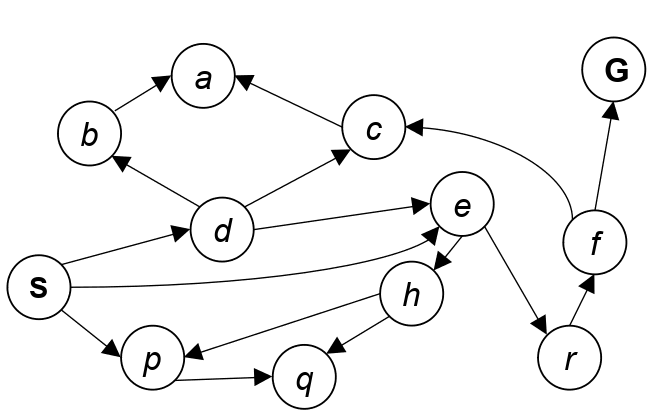
\includegraphics[width=6cm,height = 4cm]{./images/tiny_graphe.png}
  \vspace*{1cm}
  \begin{itemize}
    \item \textbf{Stratégie} : Développer le noeuds le plus
      \alert{\textbf{profond}}. 
    \item \textbf{Implémentation}: Frontière est une
      \textbf{\structure{PILE}}(LIFO). 
  \end{itemize}
\end{frame}

\begin{frame}[t]{Quiz}
 
  \begin{figure}[htpb]
  \begin{center}
  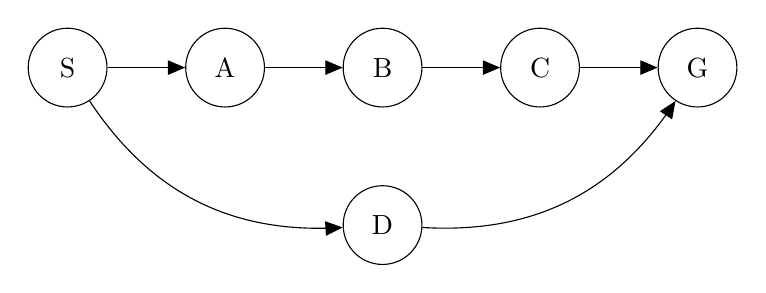
\begin{tikzpicture}[scale=1, transform shape]
    \node[draw, minimum width=1cm,circle] (S) at (0,0) {S}; 
    \node[draw, minimum width=1cm,circle] (A) at (2,0) {A}; 
    \node[draw, minimum width=1cm,circle] (B) at (4,0) {B}; 
    \node[draw, minimum width=1cm,circle] (C) at (6,0) {C}; 
    \node[draw, minimum width=1cm,circle] (G) at (8,0) {G}; 
    \node[draw, minimum width=1cm,circle] (D) at (4,-2) {D}; 
    \path[draw,->] (S)--(A);
      \path[draw,->](A)--(B);
    \path[draw,->](B)--(C);
      \path[draw,->](C)--(G);
      \path[draw,->] (S)   to [bend right=30](D);
      \path[draw,->](D) to [bend right = 30](G);
  \end{tikzpicture}
  \end{center}
  \end{figure}
  
  \begin{block}{Question}
    Donner le chemin calculé par \textbf{DPS} de son exploration du point
    $\mathbf{S}$ jusqu'au point $\mathbf{G}$. 
  \end{block}
\end{frame}


\begin{frame}[t]{Propriété d'un algorithme d'exploration}
 \begin{columns}
   \begin{column}{0.5\textwidth}
     \begin{itemize}
       \small
       \item<1-> \textbf{Complet}: Assure de trouver une solution s'il elle
       existe. 
     \item<2-> \textbf{Optimal} : Trouve la solution avec un \alert{coût}
       minimal.
      \item<3-> \textbf{Complexité en temps} 
      \item<4-> \textbf{Complexité en espace} 
     \end{itemize} 

     \begin{itemize}
       \item \structure{\textbf{Arbre d'exploration}}:
         \begin{itemize}
           \small
           \item<5-> $\mathbf{b}$ : facteur de 
           \item<6->$\mathbf{m}$ : profondeur de l'arbre.
          \item<7-> Solutions dans differents \textbf{profondeurs} 
         \end{itemize}
       \item<8->
\textbf{Nombre de noeuds} :
          \scriptsize 
          $$ 1 + b^2 + b^3 + \ldots +b^m = \alert{\mathcal{O}(b^m)}$$
     \end{itemize}
   \end{column}
   \begin{column}{0.5\textwidth}
     \begin{figure}[htpb]
     \begin{center}
     \begin{tikzpicture}[scale=1, >=stealth]
       only<4->{
         \path[draw] (0,0)--(2,-4)--(-2,-4)--cycle ;
       }   
       \only<4->{
         \node[circle,minimum width=5pt,draw,fill=lightBlue,inner sep=0pt] at (0,0) {};
         \node at (2.2,-0) { \tiny $1$ noeuds};
       }
       \only<5->
       {
         \node[circle,minimum width=5pt,draw,fill=lightBlue,inner sep=0pt] at
           (-0.25,-0.5) {};
         \node[circle,minimum width=5pt,draw,fill=lightBlue,inner sep=0pt] at
           (0.25,-0.5) {};
         \node at (2.2,-0.5) {\tiny $b$ noeuds};
         \path[->,draw,] (-0.25,-0.5) to[bend right=30]node[label=below: $b$] {} (0.25,-0.5);
       }

       \only<6->{
         \path[draw,thick,->] (-2.5,0) --node[label=left:$\mathbf{m}$]{} (-2.5,-4);

         \node at (2.2,-1) {\tiny $b^2$ noeuds};
         \node at (2.2,-1.5) {\tiny $b^3$ noeuds};
         \node at (2.2,-4.2) {\tiny $b^m$ noeuds};

  }

  \only<7->{
         %optimal nodes
         \node[circle,minimum width=5pt,draw,fill=sexyRed,inner sep=0pt] at
           (0.5,-2.5) {};

         \node[circle,minimum width=5pt,draw,fill=sexyRed,inner sep=0pt] at
           (0.1,-4) {};
       }
     \end{tikzpicture}
     \end{center}
     \end{figure}
   \end{column}
 \end{columns} 
\end{frame}



\begin{frame}[t]{Propriétés DFS}
  
 \begin{columns}
   \begin{column}{0.5\textwidth}
     \begin{itemize}
       \small
     \item \textbf{Noeuds visitées par DPS}:
         \begin{itemize}
         \scriptsize
       \item Noeuds à \textbf{gauche}.
           \item Peut visiter \textbf{toute} l'arbre
           \item Si $m$ est fini, Temps est \alert{$\mathcal{O}(b^m)$} 
         \end{itemize}
       \item \textbf{Taille de la frontière}:
         \begin{itemize}
           \scriptsize
         \item<2-> \alert{$\mathcal{O}(bm)$}
         \end{itemize}

       \item \textbf{Est il complet}?:
           \begin{itemize}
             \scriptsize
             \item Au cas où on as pas de \alert{\textbf{cycle}}.
           \end{itemize}
         \item \textbf{Est il optimal}?
            \begin{itemize}
              \scriptsize
            \item \textbf{\alert{No}} trouve toujours  le nouds à gauche
              (indépendemment du coût).
            \end{itemize}
     \end{itemize}
   \end{column}
   \begin{column}{0.5\textwidth}
     \begin{figure}[htpb]
     \begin{center}
     \begin{tikzpicture}[scale=1, >=stealth]
      
         \path[draw] (0,0)--(2,-4)--(-2,-4)--cycle ;
         \node[circle,minimum width=5pt,draw,fill=lightBlue,inner sep=0pt] at (0,0) {};
         \node[circle,minimum width=5pt,draw,fill=lightBlue,inner sep=0pt] at
           (-0.25,-0.5) {};
         \node[circle,minimum width=5pt,draw,fill=lightBlue,inner sep=0pt] at
           (0.25,-0.5) {};
         \path[->,draw,] (-0.25,-0.5) to[bend right=30]node[label=below: $b$] {} (0.25,-0.5);

         %optimal nodes
         \node[circle,minimum width=5pt,draw,fill=sexyRed,inner sep=0pt] at
           (0.5,-2.5) {};
         \node[circle,minimum width=5pt,draw,fill=sexyRed,inner sep=0pt] at
           (0.1,-4) {};
         \path[fill=gray!70,draw,thick,opacity=0.5] (0,0)--(-1.4,-4)--(-2,-4)--cycle;
         \path[fill=gray!50,draw,thick,opacity=0.5] (0,0)--(-0.9,-4)--(-1.4,-4)--cycle;
         \path[fill=gray!30,draw,thick,opacity=0.5] (0,0)--(0.1,-4)--(-0.9,-4)--cycle;
         \only<2->{\path[draw, very thick, sexyRed](0,0)--(0.1,-4);}
     \end{tikzpicture}
     \end{center}
     \end{figure}
   \end{column}
 \end{columns} 
\end{frame}
%%%%%%%%%%%%%%%%%%%%%%%%%%
%  Recherche en largeur  %
%%%%%%%%%%%%%%%%%%%%%%%%%%
\subsection{Recherche en largeur (BFS)}%
\label{sub:recherche_en_largeur_bfs_}
\begin{frame}[t]{Breadth First Search (BFS)}
 \centering 
 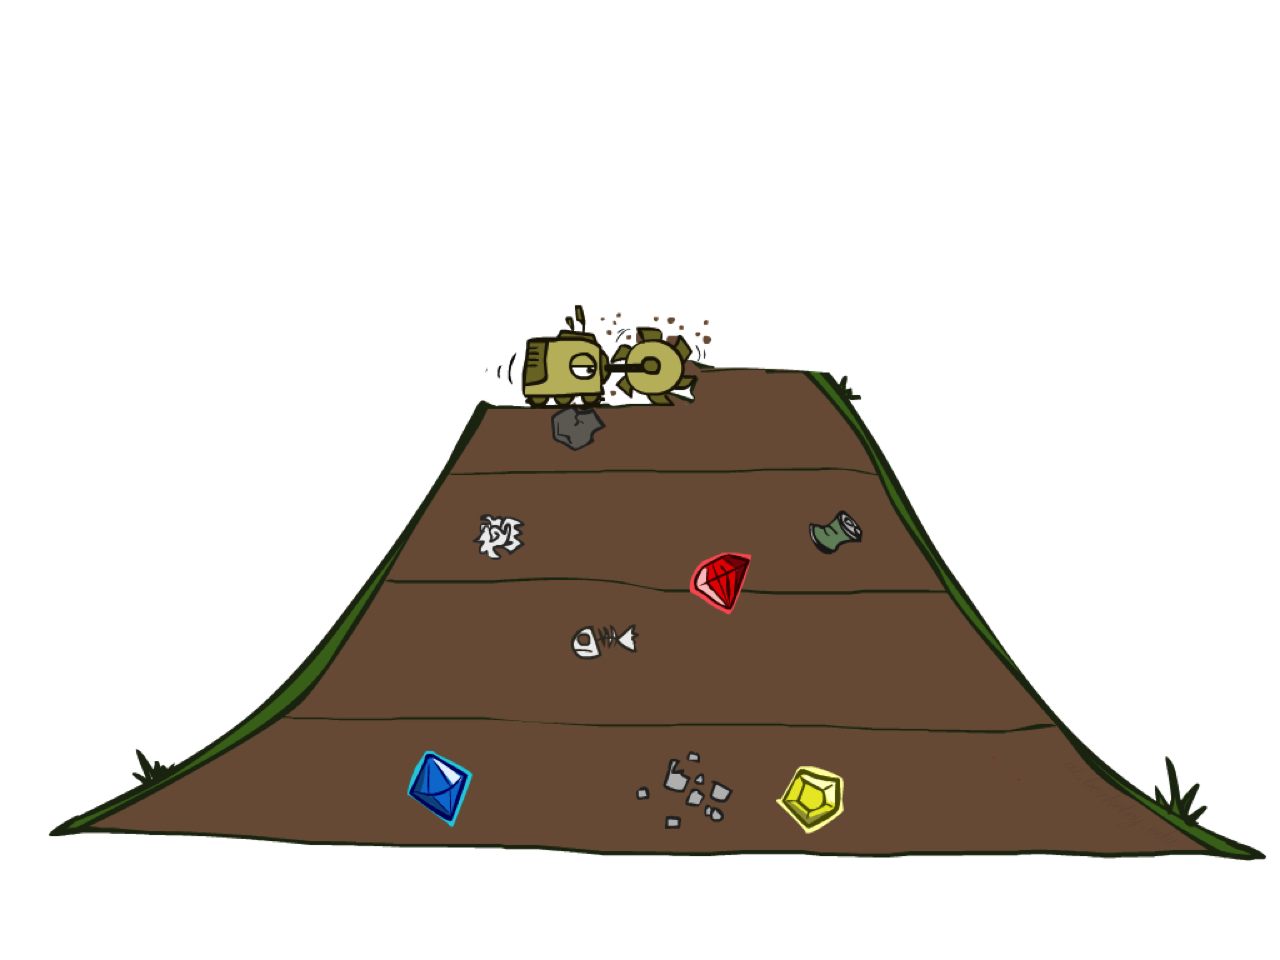
\includegraphics[width=10cm,height=6cm]{./images/breath_first_search.png}
\end{frame}

\begin{frame}[t]{BFS (Recherche en largeur)}
 \centering 
 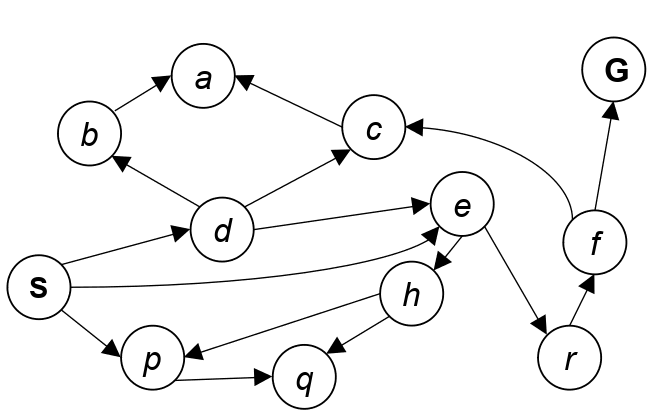
\includegraphics[width=5cm,height=4cm]{./images/tiny_graphe.png}

 \vspace*{1cm}
 \begin{block}{Propriétés}
    \begin{itemize}
      \small
    \item \textbf{Stratégie}:Developper les noeuds  \alert{superficiels}
    \item \textbf{Frontière} : est une \alert{File} (FIFO).
    \end{itemize} 
 \end{block}

\end{frame}

\begin{frame}[t]{Quiz}
 
  \begin{figure}[htpb]
  \begin{center}
  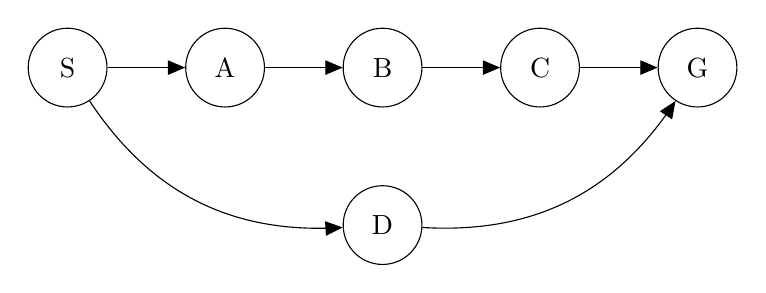
\begin{tikzpicture}[scale=1, transform shape]
    \node[draw, minimum width=1cm,circle] (S) at (0,0) {S}; 
    \node[draw, minimum width=1cm,circle] (A) at (2,0) {A}; 
    \node[draw, minimum width=1cm,circle] (B) at (4,0) {B}; 
    \node[draw, minimum width=1cm,circle] (C) at (6,0) {C}; 
    \node[draw, minimum width=1cm,circle] (G) at (8,0) {G}; 
    \node[draw, minimum width=1cm,circle] (D) at (4,-2) {D}; 
    \path[draw,->] (S)--(A);
      \path[draw,->](A)--(B);
    \path[draw,->](B)--(C);
      \path[draw,->](C)--(G);
      \path[draw,->] (S)   to [bend right=30](D);
      \path[draw,->](D) to [bend right = 30](G);
  \end{tikzpicture}
  \end{center}
  \end{figure}
  
  \begin{block}{Question}
    Donner le chemin calculé par \textbf{BPS} de son exploration du point
    $\mathbf{S}$ jusqu'au point $\mathbf{G}$. 
  \end{block}
\end{frame}
\begin{frame}[t]{Propriétés BFS}

 \begin{columns}
   \begin{column}{0.5\textwidth}
     \begin{itemize}
       \small
     \item \textbf{Noeuds visitées par BPS}:
         \begin{itemize}
         \scriptsize
       \item Tous les noeuds d'une superficie.
       \item Si $m$ est fini, Temps est \alert{$\mathcal{O}(b^s)$} 
       \item \alert{$s$} est la pronfondeur de la solution.
         \end{itemize}
       \item \textbf{Taille de la frontière}:
         \begin{itemize}
           \scriptsize
         \item<2-> \alert{$\mathcal{O}(b^s)$}
         \end{itemize}

       \item \textbf{Est il complet}?:
           \begin{itemize}
             \scriptsize
           \item Si une solution existe, $s$ est fini. Donc \alert{Oui}.
           \end{itemize}
         \item \textbf{Est il optimal}?
            \begin{itemize}
              \scriptsize
            \item \textbf{\alert{OUI}} Si tous les coûts sont $\mathbf{1}$.
            \end{itemize}
     \end{itemize}
   \end{column}
   \begin{column}{0.5\textwidth}
     \begin{figure}[htpb]
     \begin{center}
     \begin{tikzpicture}[scale=1, >=stealth]
      
         \path[draw] (0,0)--(2,-4)--(-2,-4)--cycle ;
         \node[circle,minimum width=5pt,draw,fill=lightBlue,inner sep=0pt] at (0,0) {};
         \node[circle,minimum width=5pt,draw,fill=lightBlue,inner sep=0pt] at
           (-0.25,-0.5) {};
         \node[circle,minimum width=5pt,draw,fill=lightBlue,inner sep=0pt] at
           (0.25,-0.5) {};
         \path[->,draw,] (-0.25,-0.5) to[bend right=30]node[label=below: $b$] {} (0.25,-0.5);

         %optimal nodes
         \node[circle,minimum width=5pt,draw,fill=sexyRed,inner sep=0pt] at
           (0.5,-3) {};
         \node[circle,minimum width=5pt,draw,fill=sexyRed,inner sep=0pt] at
           (0.1,-4) {};

         %areas
         \path[fill=gray!70,draw,thick,opacity=0.5]
           (0,0)--(-0.25,-0.5)--(0.25,-0.5)--cycle;
         \path[fill=gray!80,draw,thick,opacity=0.5]
           (-0.25,-0.5)--(-0.5,-1)--(0.5,-1)--(0.25,-0.5)--cycle;
         \path[fill=gray!90,draw,thick,opacity=0.5]
           (-0.5,-1)--(-1.5,-3)--(1.5,-3)--(0.5,-1)--cycle;
         \path[draw,thick] (-1,-2)--(1,-2);
     \end{tikzpicture}
     \end{center}
     \end{figure}
   \end{column}
 \end{columns} 
\end{frame}
%%%%%%%%%%%%%%%%%%%%%%%%%
%  Uniform cost search  %
%%%%%%%%%%%%%%%%%%%%%%%%%
\subsection{Recherche uniforme en coût (UCS)}%
\label{sub:recherche_uniforme_en_cout_ucs_}
\begin{frame}[t]{Recherche uniforme en coût}
  
\end{frame}











\end{document}
